\section{Sprint 2 - Transaction Management}

\subsection{Use Case Diagram}

The following diagram illustrates the main use cases implemented during Sprint 2, showing the interactions between End Users and the transaction management system, focusing on barcode generation, payment processing, and transaction history management.

\begin{figure}[H]
\centering
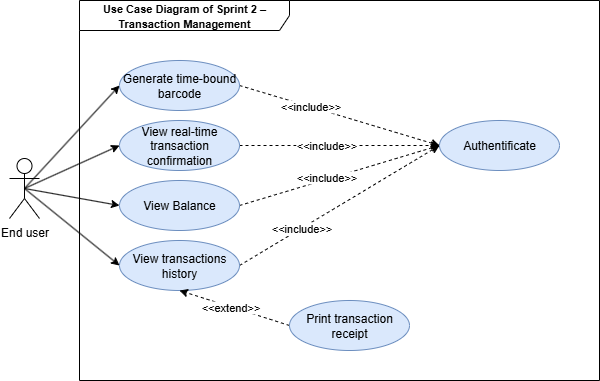
\includegraphics[width=0.9\textwidth]{images/usecase_sprint2.png}
\caption{Sprint 2 Use Case Diagram - Transaction Management}
\label{fig:sprint2_usecase_diagram}
\end{figure}

\subsection{Use Case Descriptions}

\subsubsection{UC4: Generate Time-bound Barcode}

\begin{longtable}{|p{3cm}|p{11cm}|}
\hline
\textbf{Use Case ID} & UC4 \\
\hline
\textbf{Use Case Name} & Generate Time-bound Barcode \\
\hline
\textbf{Description} & This use case allows end users to generate a secure, time-bound barcode containing their wallet's tokenizedId for payment processing at vendor locations. \\
\hline
\textbf{Primary Actor} & End User \\
\hline
\textbf{Secondary Actor} & Wallet System, Barcode Generator \\
\hline
\textbf{Preconditions} & 
\begin{itemize}[nosep,leftmargin=*]
\item End user is authenticated and has access to their wallet
\item Wallet exists and is active in the system
\item Mobile device has barcode display capability
\end{itemize} \\
\hline
\textbf{Postconditions} & 
\begin{itemize}[nosep,leftmargin=*]
\item Time-bound barcode is generated using wallet's tokenizedId
\item Barcode expires after 30 seconds for security
\item User can present barcode to vendor for scanning
\end{itemize} \\
\hline
\textbf{Main Flow} & 
\begin{enumerate}[nosep,leftmargin=*]
\item End user opens wallet application and navigates to payment section
\item User selects "Generate Payment Barcode" option
\item System retrieves user's wallet tokenizedId from database
\item System generates Code128 barcode encoding the tokenizedId
\item System displays barcode on screen with 30-second countdown timer
\item User presents device screen to vendor for barcode scanning
\item Barcode automatically expires after 30 seconds for security
\item User can regenerate new barcode if needed
\end{enumerate} \\
\hline
\textbf{Alternative Flow} & 
\begin{itemize}[nosep,leftmargin=*]
\item \textbf{A1:} Barcode expires - User can generate new barcode immediately
\item \textbf{A2:} Screen brightness adjustment - System automatically increases brightness for better scanning
\item \textbf{A3:} Multiple payment attempts - User can generate multiple barcodes in sequence
\end{itemize} \\
\hline
\textbf{Exception Flow} & 
\begin{itemize}[nosep,leftmargin=*]
\item \textbf{E1:} Wallet not found - System displays error and redirects to wallet setup
\item \textbf{E2:} Network connectivity issues - System displays cached wallet information with warning
\item \textbf{E3:} Insufficient balance - System displays balance warning but still generates barcode
\end{itemize} \\
\hline
\end{longtable}

\subsubsection{UC5: View Real-time Transaction Confirmation}

\begin{longtable}{|p{3cm}|p{11cm}|}
\hline
\textbf{Use Case ID} & UC5 \\
\hline
\textbf{Use Case Name} & View Real-time Transaction Confirmation \\
\hline
\textbf{Description} & This use case provides end users with immediate confirmation and detailed information about completed payment transactions. \\
\hline
\textbf{Primary Actor} & End User \\
\hline
\textbf{Secondary Actor} & Transaction System, ASM POS Integration \\
\hline
\textbf{Preconditions} & 
\begin{itemize}[nosep,leftmargin=*]
\item User has initiated a payment transaction
\item Vendor has scanned user's barcode
\item Payment processing is in progress
\end{itemize} \\
\hline
\textbf{Postconditions} & 
\begin{itemize}[nosep,leftmargin=*]
\item User receives immediate transaction confirmation
\item Wallet balance is updated in real-time
\item Transaction is recorded in user's history
\end{itemize} \\
\hline
\textbf{Main Flow} & 
\begin{enumerate}[nosep,leftmargin=*]
\item User presents barcode to vendor for scanning
\item Vendor scans barcode and enters transaction amount
\item System processes payment through ASM POS integration
\item System validates transaction and updates wallet balance
\item User receives real-time notification of successful payment
\item System displays transaction confirmation with details (amount, timestamp, vendor, balance)
\item User can view digital receipt immediately
\end{enumerate} \\
\hline
\textbf{Alternative Flow} & 
\begin{itemize}[nosep,leftmargin=*]
\item \textbf{A1:} Slow network connection - System shows processing indicator
\item \textbf{A2:} Partial payment - System handles split transactions
\end{itemize} \\
\hline
\textbf{Exception Flow} & 
\begin{itemize}[nosep,leftmargin=*]
\item \textbf{E1:} Payment declined - System displays reason and suggests alternatives
\item \textbf{E2:} Network timeout - System queues transaction for retry
\item \textbf{E3:} Insufficient funds - System displays balance error and cancels transaction
\end{itemize} \\
\hline
\end{longtable}

\subsubsection{UC6: View Balance}

\begin{longtable}{|p{3cm}|p{11cm}|}
\hline
\textbf{Use Case ID} & UC6 \\
\hline
\textbf{Use Case Name} & View Balance \\
\hline
\textbf{Description} & This use case allows end users to view their current wallet balance with real-time updates and refresh capabilities. \\
\hline
\textbf{Primary Actor} & End User \\
\hline
\textbf{Secondary Actor} & Wallet System, Database \\
\hline
\textbf{Preconditions} & 
\begin{itemize}[nosep,leftmargin=*]
\item User is authenticated and has access to wallet
\item Wallet exists and is active in the system
\end{itemize} \\
\hline
\textbf{Postconditions} & 
\begin{itemize}[nosep,leftmargin=*]
\item Current wallet balance is displayed accurately
\item Balance information is refreshed from server
\item User has visibility into available funds
\end{itemize} \\
\hline
\textbf{Main Flow} & 
\begin{enumerate}[nosep,leftmargin=*]
\item User opens wallet application home screen
\item System automatically retrieves current wallet balance
\item System displays balance prominently on home interface
\item User can pull-to-refresh to update balance manually
\item System shows last updated timestamp for transparency
\item Balance updates automatically after transactions
\end{enumerate} \\
\hline
\textbf{Alternative Flow} & 
\begin{itemize}[nosep,leftmargin=*]
\item \textbf{A1:} Offline mode - System displays last cached balance with indicator
\item \textbf{A2:} Multiple currency support - System displays balance in preferred currency
\end{itemize} \\
\hline
\textbf{Exception Flow} & 
\begin{itemize}[nosep,leftmargin=*]
\item \textbf{E1:} Balance retrieval failure - System displays cached balance with error indicator
\item \textbf{E2:} Wallet suspended - System displays suspension notice
\end{itemize} \\
\hline
\end{longtable}

\subsubsection{UC7: View Transactions History}

\begin{longtable}{|p{3cm}|p{11cm}|}
\hline
\textbf{Use Case ID} & UC7 \\
\hline
\textbf{Use Case Name} & View Transactions History \\
\hline
\textbf{Description} & This use case provides end users with comprehensive access to their complete transaction history with filtering and search capabilities. \\
\hline
\textbf{Primary Actor} & End User \\
\hline
\textbf{Secondary Actor} & Transaction System, Database \\
\hline
\textbf{Preconditions} & 
\begin{itemize}[nosep,leftmargin=*]
\item User is authenticated and has wallet access
\item User has performed at least one transaction (or none for empty state)
\end{itemize} \\
\hline
\textbf{Postconditions} & 
\begin{itemize}[nosep,leftmargin=*]
\item Complete transaction history is displayed chronologically
\item User can access detailed information for each transaction
\item Transaction data is properly formatted and searchable
\end{itemize} \\
\hline
\textbf{Main Flow} & 
\begin{enumerate}[nosep,leftmargin=*]
\item User navigates to "Transaction History" from main menu
\item System retrieves all transactions associated with user's wallet
\item System displays transactions in reverse chronological order
\item Each transaction shows: date, amount, vendor, status, and type
\item User can tap on any transaction to view detailed information
\item Detailed view includes: transaction ID, timestamp, description, receipt
\item User can filter transactions by date range, amount, or vendor
\item User can search transactions using keywords
\end{enumerate} \\
\hline
\textbf{Alternative Flow} & 
\begin{itemize}[nosep,leftmargin=*]
\item \textbf{A1:} No transactions - System displays empty state with helpful guidance
\item \textbf{A2:} Large transaction history - System implements pagination for performance
\item \textbf{A3:} Export functionality - User can export transaction history as PDF/CSV
\end{itemize} \\
\hline
\textbf{Exception Flow} & 
\begin{itemize}[nosep,leftmargin=*]
\item \textbf{E1:} Data loading failure - System displays cached transactions with sync indicator
\item \textbf{E2:} Corrupted transaction data - System displays available information with error notice
\item \textbf{E3:} Network timeout - System shows retry option with offline data
\end{itemize} \\
\hline
\end{longtable}

\subsection{Sequence Diagrams}

\subsubsection{View Balance Sequence Diagram}

This diagram illustrates the process of retrieving and displaying wallet balance. The end user requests balance information through the home interface, which communicates with the wallet controller to fetch current balance data from the wallet entity and display it to the user.

\begin{figure}[H]
\centering
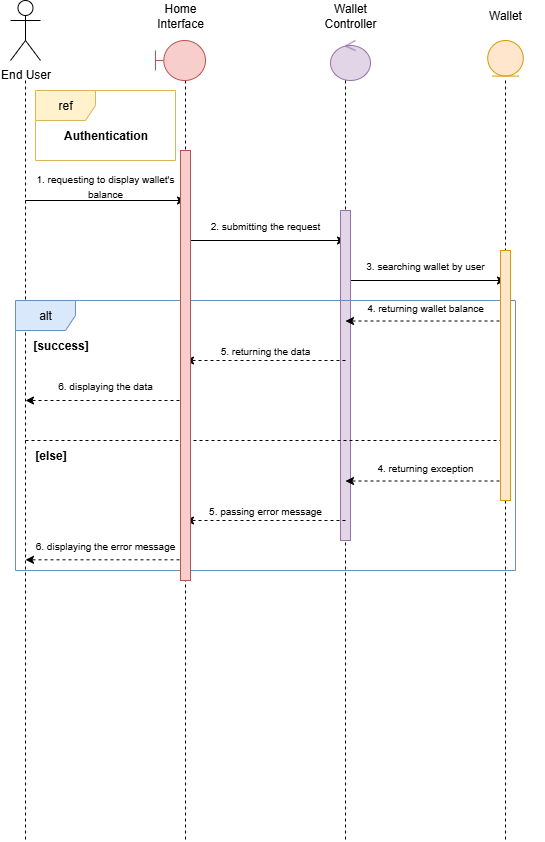
\includegraphics[width=0.9\textwidth]{images/seq_view_balance.png}
\caption{View Balance Sequence Diagram}
\label{fig:seq_view_balance}
\end{figure}

\subsubsection{View Transactions Sequence Diagram}

This diagram shows the transaction history retrieval process. The end user requests transaction history through the transactions interface, which communicates with the transaction controller to fetch transaction data from the transaction entity and display the chronological list to the user.

\begin{figure}[H]
\centering
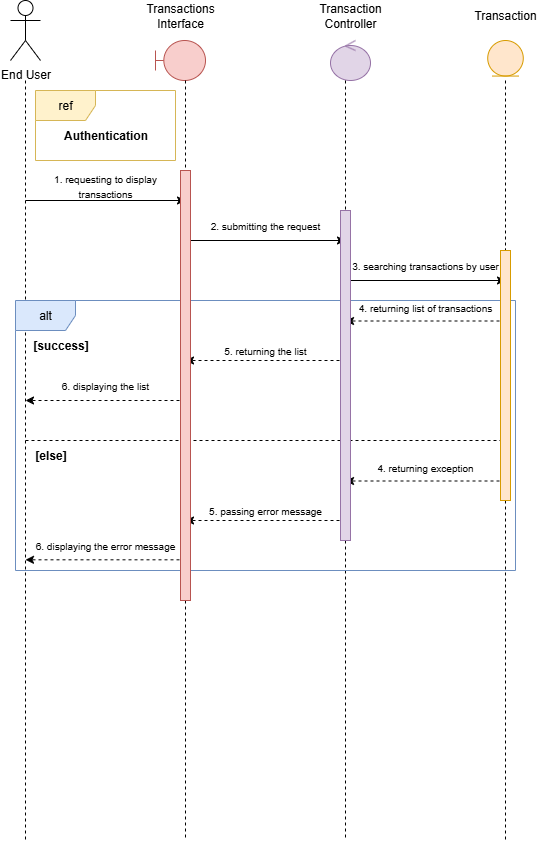
\includegraphics[width=0.9\textwidth]{images/seq_view_transactions.png}
\caption{View Transactions Sequence Diagram}
\label{fig:seq_view_transactions}
\end{figure}

\subsection{Class Diagram}

The Sprint 2 class diagram extends the foundational entities from Sprint 1 with transaction management capabilities, showing the relationships between User, Corporate, Wallet, Transaction, TransactionType, and TransactionStatus entities.

\begin{figure}[H]
\centering
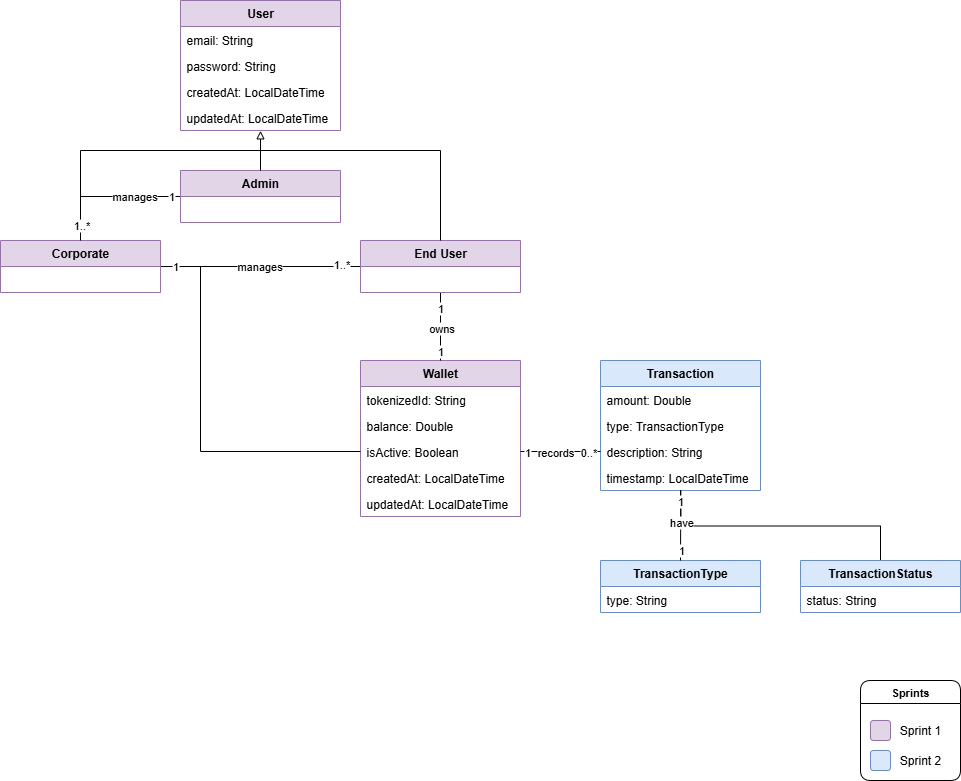
\includegraphics[width=0.9\textwidth]{images/class_sprint2.png}
\caption{Class Diagram - Sprint 2}
\label{fig:class_sprint2}
\end{figure}

\subsection{Realization}

This section presents the actual implementation of Sprint 2 use cases through screenshots of the developed Flutter mobile application and web admin portal.

\subsubsection{UC4: Generate Time-bound Barcode - Realization}

The barcode generation interface provides secure, time-bound payment codes for vendor scanning. The implementation includes Code128 barcode generation using the wallet's tokenizedId with a 30-second expiry timer.

% \begin{figure}[H]
% \centering
% \includegraphics[width=0.6\textwidth]{images/barcode_generation_screen.png}
% \caption{Barcode Generation Screen - Flutter Mobile App}
% \label{fig:barcode_generation_realization}
% \end{figure}

\subsubsection{UC6: View Balance - Realization}

The wallet balance interface displays the current balance prominently on the home screen with real-time updates and pull-to-refresh functionality.

% \begin{figure}[H]
% \centering
% \includegraphics[width=0.6\textwidth]{images/home_balance_screen.png}
% \caption{Home Screen with Balance Display - Flutter Mobile App}
% \label{fig:balance_view_realization}
% \end{figure}

\subsubsection{UC7: View Transactions History - Realization}

The transaction history interface provides comprehensive transaction management with chronological listing and detailed transaction information.

% \begin{figure}[H]
% \centering
% \includegraphics[width=0.6\textwidth]{images/transaction_history_screen.png}
% \caption{Transaction History Screen - Flutter Mobile App}
% \label{fig:transaction_history_realization}
% \end{figure}
